% \DeclareDocumentMetadata {lang=en-US}

% xmp metadata for pdf
% Originally used \usepackage[a-2a]{pdfx}
% \usepackage{hyperxmp} replaced it
% \RequirePackage{pdfmanagement-testphase} replaced it
% \PassOptionsToPackage{enable-debug,check-declarations}{expl3} broke with version 0.9 of tagpdf
% \ExplSyntaxOn no need for these 3 lines because metadata can handle it
% \pdfmanagement_add:nnn{Catalog}{Lang}{(enUS)} enUS is wrong, should be en-US
% \ExplSyntaxOff

\documentclass[11pt,
  english,
  letterpaper,
]{article}
\usepackage{sa4ss}
\usepackage{amsmath,amssymb,array}
\usepackage{booktabs}

% From tagged-template.latex
\usepackage{lmodern}
\usepackage{ifxetex,ifluatex}
\ifnum 0\ifxetex 1\fi\ifluatex 1\fi=0 % if pdftex
  \usepackage[T1]{fontenc}
  \usepackage[utf8]{inputenc}
  \usepackage{textcomp} % provide euro and other symbols
\else % if luatex or xetex
  \usepackage{unicode-math}
  \defaultfontfeatures{Scale=MatchLowercase}
  \defaultfontfeatures[\rmfamily]{Ligatures=TeX,Scale=1}
\fi

% Use upquote if available, for straight quotes in verbatim environments
\IfFileExists{upquote.sty}{\usepackage{upquote}}{}
\IfFileExists{microtype.sty}{% use microtype if available
  \usepackage[]{microtype}
  \UseMicrotypeSet[protrusion]{basicmath} % disable protrusion for tt fonts
}{}
\makeatletter
\@ifundefined{KOMAClassName}{% if non-KOMA class
  \IfFileExists{parskip.sty}{%
    \usepackage{parskip}
  }{% else
    \setlength{\parindent}{0pt}
    \setlength{\parskip}{6pt plus 2pt minus 1pt}}
}{% if KOMA class
  \KOMAoptions{parskip=half}}
\makeatother
\usepackage{xcolor}
\IfFileExists{xurl.sty}{\usepackage{xurl}}{} % add URL line breaks if available
\hypersetup{
  pdftitle={Status of Shortspine Thornyhead (Sebastolobus alascanus) along the US West coast in 2023},
  pdflang={en},
  hidelinks,
  pdfcreator={LaTeX via pandoc}}
\urlstyle{same} % disable monospaced font for URLs
\usepackage{longtable}
% Correct order of tables after \paragraph or \subparagraph
\usepackage{etoolbox}
\makeatletter
\patchcmd\longtable{\par}{\if@noskipsec\mbox{}\fi\par}{}{}
\makeatother
% Allow footnotes in longtable head/foot
\IfFileExists{footnotehyper.sty}{\usepackage{footnotehyper}}{\usepackage{footnote}}
\makesavenoteenv{longtable}
\usepackage{graphicx}
\makeatletter
\def\maxwidth{\ifdim\Gin@nat@width>\linewidth\linewidth\else\Gin@nat@width\fi}
\def\maxheight{\ifdim\Gin@nat@height>\textheight\textheight\else\Gin@nat@height\fi}
\makeatother
% Scale images if necessary, so that they will not overflow the page
% margins by default, and it is still possible to overwrite the defaults
% using explicit options in \includegraphics[width, height, ...]{}
\setkeys{Gin}{width=\maxwidth,height=\maxheight,keepaspectratio}
% Set default figure placement to htbp
\makeatletter
\def\fps@figure{htbp}
\makeatother
\setlength{\emergencystretch}{3em} % prevent overfull lines
\providecommand{\tightlist}{%
  \setlength{\itemsep}{0pt}\setlength{\parskip}{0pt}}
\setcounter{secnumdepth}{5}
\ifxetex
  % Load polyglossia as late as possible: uses bidi with RTL langages (e.g. Hebrew, Arabic)
  \usepackage{polyglossia}
  \setmainlanguage[]{}
\else
  \usepackage[shorthands=off,main=english]{babel}
\fi

%Define cslreferences environment, required by pandoc 2.8
%https://github.com/rstudio/rmarkdown/issues/1649
\newlength{\csllabelwidth}
\setlength{\csllabelwidth}{3em}
\newlength{\cslhangindent}
\setlength{\cslhangindent}{1.5em}
% for Pandoc 2.8 to 2.10.1
\newenvironment{cslreferences}%
  {}%
  {\par}
% For Pandoc 2.11+
\newenvironment{CSLReferences}[2] % #1 hanging-ident, #2 entry spacing
 {% don't indent paragraphs
  \setlength{\parindent}{0pt}
  % turn on hanging indent if param 1 is 1
  \ifodd #1 \everypar{\setlength{\hangindent}{\cslhangindent}}\ignorespaces\fi
  % set entry spacing
  \ifnum #2 > 0
  \setlength{\parskip}{#2\baselineskip}
  \fi
 }%
 {}
\usepackage{calc}  % for \widthof, \maxof in minipage
\newcommand{\CSLBlock}[1]{#1\hfill\break}
\newcommand{\CSLLeftMargin}[1]{\parbox[t]{\csllabelwidth}{#1}}
\newcommand{\CSLRightInline}[1]{\parbox[t]{\linewidth - \csllabelwidth}{#1}\break}
\newcommand{\CSLIndent}[1]{\hspace{\cslhangindent}#1}


\providecommand{\tightlist}{%
  \setlength{\itemsep}{0pt}\setlength{\parskip}{0pt}}


\date{}
\newcommand{\trTitle}{Status of Shortspine Thornyhead (\emph{Sebastolobus alascanus}) along the US West coast in 2023}
\newcommand{\trYear}{2023}
\newcommand{\trMonth}{April}
\newcommand{\trAuthsLong}{truetruetruetruetruetruetruetruetrue}
\newcommand{\trAuthsBack}{Shipley, M., J. Zahner, S. Beyer, A. Hayes, P.-. Hernvann, A. Odell, H. Oleynik, J.Y. Sullivan, M. Veron}
\newcommand{\trCitation}{
\begin{hangparas}{1em}{1}
\trAuthsBack{}. \trYear{}. \trTitle{}. \glsentrylong{pfmc}, Portland, Oregon. \pageref{LastPage}{}\,p.
\end{hangparas}}

\begin{document}

%%%%% Frontmatter %%%%%

% Footnote symbols in front matter
\renewcommand*{\thefootnote}{\fnsymbol{footnote}}

\small
\thispagestyle{empty}
\pagenumbering{roman}
\noindent
\begin{center}
\title{Status of Shortspine Thornyhead (\emph{Sebastolobus alascanus}) along the US West coast in 2023}
% \textnormal{\MakeTextUppercase{\trTitle{}}}
\vspace{1.5cm}
{\Large\textbf\newline{Status of Shortspine Thornyhead (\emph{Sebastolobus alascanus}) along the US West coast in 2023}}
\vfill
by\\
Madison Shipley\textsuperscript{1}\\
Joshua Zahner\textsuperscript{1}\\
Sabrina Beyer\textsuperscript{1}\\
Adam Hayes\textsuperscript{1}\\
Pierre-Yves Hernvann\textsuperscript{2}\\
Andrea Odell\textsuperscript{3}\\
Haley Oleynik\textsuperscript{4}\\
Jane Y. Sullivan\textsuperscript{5}\\
Matthieu Veron\textsuperscript{6}\vfill
\textsuperscript{1}School of Aquatic and Fishery Sciences, University of Washington, 1122 NE Boat Street, Seattle, Washington 98195\\
\textsuperscript{2}Northwest Fisheries Science Center, U.S. Department of Commerce, National Oceanic and Atmospheric Administration, National Marine Fisheries Service, 2725 Montlake Boulevard East, Seattle, Washington 98112\\
\textsuperscript{3}University of California Davis, One Shields Avenue, Davis, California 95616\\
\textsuperscript{4}Institute for the Oceans and Fisheries, University of British Columbia, 2202 Main Mall, Vancouver, British Columbia Canada V6T 1Z4\\
\textsuperscript{5}Alaska Fisheries Science Center, U.S. Department of Commerce, National Oceanic and Atmospheric Administration, National Marine Fisheries Service, 17109 Point Lena Loop Road, Juneau, Alaska 99801\\
\textsuperscript{6}Alaska Fisheries Science Center, U.S. Department of Commerce, National Oceanic and Atmospheric Administration, National Marine Fisheries Service, 7600 Sand Point Way N.E., Seattle, Washington 98115\vfill
\trMonth{} \trYear{}
\end{center}
\clearpage

% Fourth page: Colophon
\thispagestyle{empty}
\vspace*{\fill}
\begin{center}
\copyright{} \glsentrylong{pfmc}, \trYear{}\\
\end{center}
\par
\bigskip
\noindent
Correct citation for this publication:
\bigskip
\par
\trCitation{}
\clearpage

% Add TOC to pdf bookmarks (clickable pdf)
\pdfbookmark[1]{\contentsname}{toc}

% Table of contents page, lists of figures and tables
\tableofcontents\clearpage
\label{TRlastRoman}
\clearpage

% Table of contents
\newpage
\thispagestyle{empty} % to remove page number

% Settings for the main document
\pagenumbering{arabic}  % Regular page numbers
\pagestyle{plain}  % No page number on first page of main document, use 'empty'
\renewcommand*{\thefootnote}{\arabic{footnote}}  % Back to numeric footnotes
\setcounter{footnote}{0}  % And start at 1
\renewcommand{\headrulewidth}{0.5pt}
\renewcommand{\footrulewidth}{0.5pt}
%\pagestyle{fancy}\fancyhead[c]{Draft: Do not cite or circulate}

\newcommand{\lt}{\ensuremath <}
\newcommand{\gt}{\ensuremath >}

\pagebreak
\pagenumbering{roman}
\setcounter{page}{1}

\renewcommand{\thetable}{\roman{table}}
\renewcommand{\thefigure}{\roman{figure}}

\setlength\parskip{0.5em plus 0.1em minus 0.2em}

\hypertarget{executive-summary}{%
\section*{Executive summary}\label{executive-summary}}
\addcontentsline{toc}{section}{Executive summary}

\hypertarget{stock}{%
\subsection*{Stock}\label{stock}}
\addcontentsline{toc}{subsection}{Stock}

This assessment reports the status of Shortspine Thornyhead (\emph{Sebastolobus alascanus}) off the US West coast using data through xxxx.

\hypertarget{catches}{%
\subsection*{Catches}\label{catches}}
\addcontentsline{toc}{subsection}{Catches}

Replace text with trends and current levels. Include Table for last 10 years. Include Figure with long-term estimates.

\hypertarget{data-and-assessment}{%
\subsection*{Data and assessment}\label{data-and-assessment}}
\addcontentsline{toc}{subsection}{Data and assessment}

This assessment uses the stock assessment framework Stock Synthesis

(SS3).

Replace text with date of last assessment, type of assessment model, data available, new information, and information lacking.

\hypertarget{stock-biomass-and-dynamics}{%
\subsection*{Stock biomass and dynamics}\label{stock-biomass-and-dynamics}}
\addcontentsline{toc}{subsection}{Stock biomass and dynamics}

Replace text with trends and current levels relative to virgin or historic levels and description of uncertainty. Include Table for last 10 years. Include Figure with long-term estimates.

\hypertarget{recruitment}{%
\subsection*{Recruitment}\label{recruitment}}
\addcontentsline{toc}{subsection}{Recruitment}

Replace text with trends and current levels relative to virgin or historic levels and description of uncertainty. Include Table for last 10 years. Include Figure with long-term estimates.

\hypertarget{exploitation-status}{%
\subsection*{Exploitation status}\label{exploitation-status}}
\addcontentsline{toc}{subsection}{Exploitation status}

Replace text with total catch divided by exploitable biomass or SPR harvest rate. Include Table for last 10 years. Include Figure with trend in f relative to target vs.~trend in biomass relative to the target.

\hypertarget{ecosystem-considerations}{%
\subsection*{Ecosystem considerations}\label{ecosystem-considerations}}
\addcontentsline{toc}{subsection}{Ecosystem considerations}

Replace text with a summary of reviewed environmental and ecosystem factors that appear to be correlated with stock dynamics. These may include variability in they physical environment, habitat, competitors, prey, or predators that directly or indirectly affects the stock's status, vital rates (growth, survival, productivity/recruitment) or range and distribution. Note which, if any, ecosystem factors are used in the assessment and how (e.g., as background information, in data preparations, as data inputs, in decisions about model structure).

\hypertarget{reference-points}\), i.e., the \(B_{MSY}\) proxy and the equilibrium stock size that results from fishing at the default harvest rate, i.e., the \(F_{MSY}\) proxy. Include Table of estimated reference points for ssb, SPR, exploitation rate, and yield based on SSB proxy for MSY, SPR proxy for MSY, and estimated MSY values.

\hypertarget{management-performance}{%
\subsection*{Management performance}\label{management-performance}}
\addcontentsline{toc}{subsection}{Management performance}

Include Table of most recent 10 years of catches in comparison with OFL, ABC, HG, and OY/ACL values, overfishing levels, actual catch and discard. Include OFL (encountered), OFL (retained), and OFL (dead) if different due to discard and discard mortality.

\hypertarget{unresolved-problems-and-major-uncertainties}{%
\subsection*{Unresolved problems and major uncertainties}\label{unresolved-problems-and-major-uncertainties}}
\addcontentsline{toc}{subsection}{Unresolved problems and major uncertainties}

Replace text with any special issues that complicate scientific assessment, questions about the best model scenario, etc.

\hypertarget{decision-table-and-projections}{%
\subsection*{Decision table and projections}\label{decision-table-and-projections}}
\addcontentsline{toc}{subsection}{Decision table and projections}

Replace text with projected yields (OFL, ABC, and ACL), spawning biomass, and stock depletion levels for each year. OFL calculations should be based on the assumption that future catches equal ABCs and not OFLs.

\hypertarget{scientific-uncertainty}{%
\subsection*{Scientific uncertainty}\label{scientific-uncertainty}}
\addcontentsline{toc}{subsection}{Scientific uncertainty}

Replace text with the sigma value and the basis for its calculation.

\hypertarget{research-and-data-needs}{%
\subsection*{Research and data needs}\label{research-and-data-needs}}
\addcontentsline{toc}{subsection}{Research and data needs}

Replace text with information gaps that seriously impede the stock assessment.

\pagebreak
\setlength{\parskip}{5mm plus1mm minus1mm}
\pagenumbering{arabic}
\setcounter{page}{1}
\renewcommand{\thefigure}{\arabic{figure}}
\renewcommand{\thetable}{\arabic{table}}
\setcounter{table}{0}
\setcounter{figure}{0}

\hypertarget{introduction}{%
\section{Introduction}\label{introduction}}

\hypertarget{basic-information}{%
\subsection{Basic Information}\label{basic-information}}

This assessment reports the status of Shortspine Thornyhead (\emph{Sebastolobus alascanus}) off the US West coast using data through xxxx.

\hypertarget{life-history}{%
\subsection{Life History}\label{life-history}}

Replace text.

\hypertarget{ecosystem-considerations-1}{%
\subsection{Ecosystem Considerations}\label{ecosystem-considerations-1}}

Replace text.

\hypertarget{historical-and-current-fishery-information}{%
\subsection{Historical and Current Fishery Information}\label{historical-and-current-fishery-information}}

Replace text.

\hypertarget{summary-of-management-history-and-performance}{%
\subsection{Summary of Management History and Performance}\label{summary-of-management-history-and-performance}}

Replace text.

\hypertarget{foreign-fisheries}{%
\subsection{Foreign Fisheries}\label{foreign-fisheries}}

Replace text.

\hypertarget{data}{%
\section{Data}\label{data}}

Data comprise the foundational components of stock assessment models. The decision to include or exclude particular data sources in an assessment model depends on many factors. These factors often include, but are not limited to, the way in which data were collected (e.g., measurement method and consistency); the spatial and temporal coverage of the data; the quantity of data available per desired sampling unit; the representativeness of the data to inform the modeled processes of importance; timing of when the data were provided; limitations imposed by the Terms of Reference; and the presence of an avenue for the inclusion of the data in the assessment model. Attributes associated with a data source can change through time, as can the applicability of the data source when different modeling approaches are explored (e.g., stock structure or time-varying processes). Therefore, the specific data sources included or excluded from this assessment should not necessarily constrain the selection of data sources applicable to future stock assessments for Shortspine Thornyhead. Even if a data source is not directly used in the stock assessment they can provide valuable insights into biology, fishery behavior, or localized dynamics.

Data from a wide range of programs were available for possible inclusion in the current assessment model. Descriptions of each data source included in the model (Figure \ref{fig:data-plot}) and sources that were explored but not included in the base model are provided below. Data that were excluded from the base model were explicitly explored during the development of this stock assessment or have not changed since their past exploration in a previous Shortspine Thornyhead stock assessment. In some cases, the inclusion of excluded data sources were explored through sensitivity analyses (see Section \ref{assessment-model}).

An overview of the data sources available for each combination of fleet and year is provided in (Figure \textbar{}(\textbf{ref?})(fig:data-plot.png))

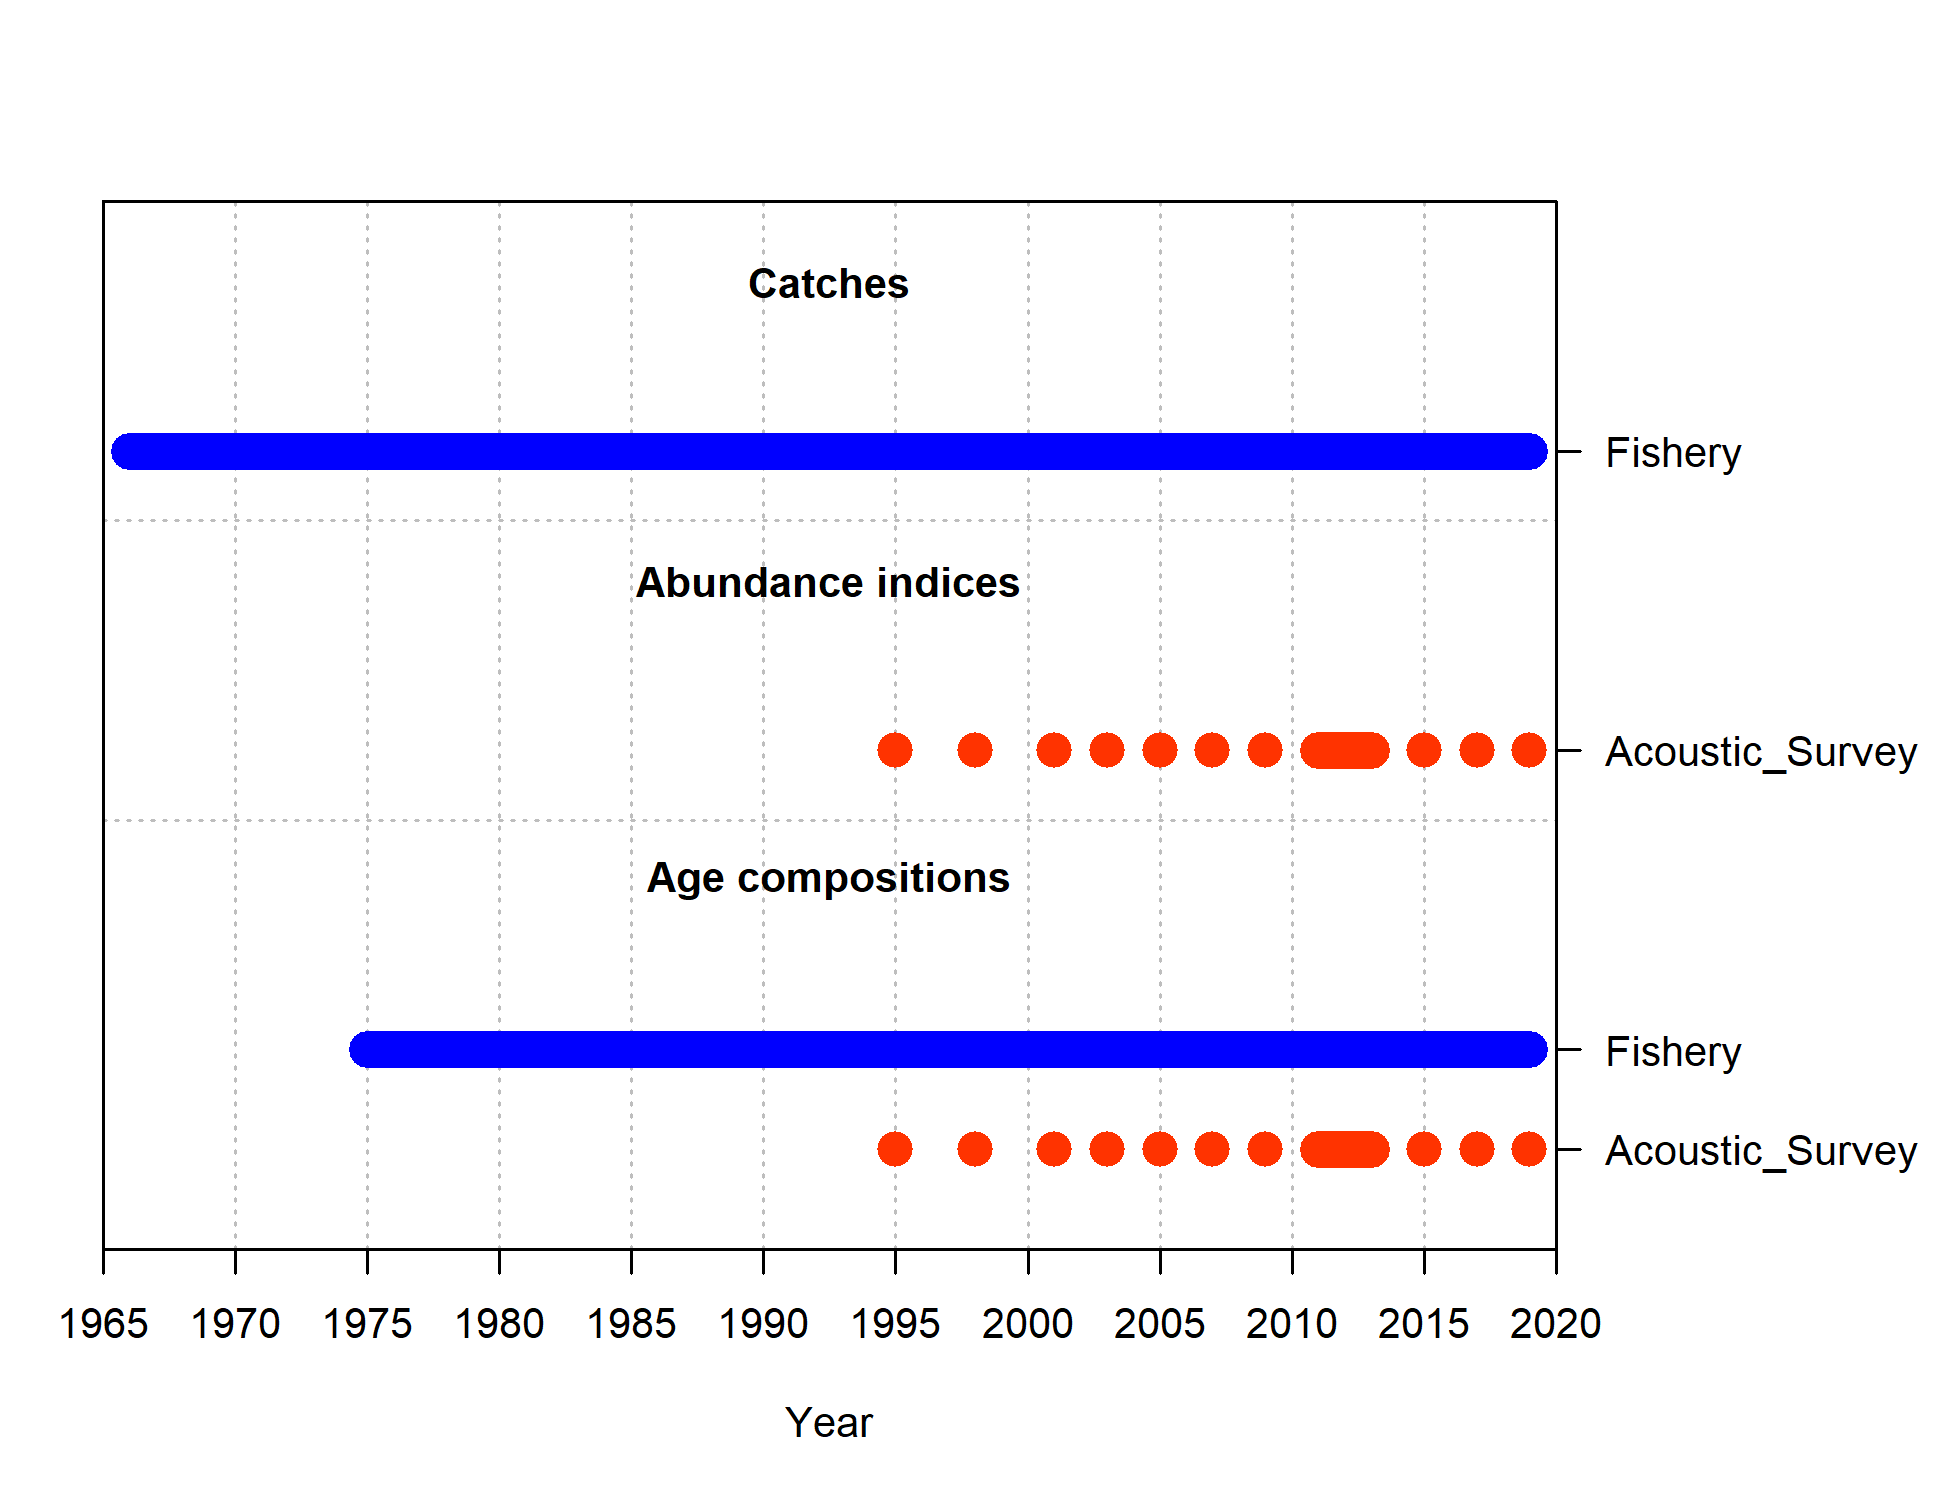
\includegraphics{data-plot.png}\{width= 100\% height=100\% alt= ``Summary of data sources used in the base model''\}

\hypertarget{biology}{%
\subsection{Biology}\label{biology}}

Shortspine Thornyhead

Shortspine Thornyhead

\gls{afsc}

\hypertarget{natural-mortality-and-longevity}{%
\subsubsection{Natural mortality and longevity}\label{natural-mortality-and-longevity}}

Butler (1995) estimated the lifespan of Shortspine Thornyhead to exceed 100 years, and suggested that M was likely less than 0.05. M may decrease with age as shortspine migrate ontogenetically down the slope to the oxygen minimum zone, which is largely devoid of predators for fish of their body size. The 2005 assessment fixed the natural mortality parameter at 0.05, while the 2013 assessment used a prior on natural mortality developed based on a maximum age of 100 years. The prior had a mean of 0.0505 and a standard deviation on a log scale of 0.5361 (Hamel, pers. comm.). For the base case, natural mortality was fixed at the mean of this prior distribution. This assessment uses an updated prior on M by Owen S. Hamel (2022), where the median of M is: \begin{equation} \frac{5.40}{Age_{max}} \end{equation}

This assessment assumed the same maximum age of 100 as in the previous assessments, with an updated prior of 0.054 (median value) and log-space standard deviation = 0.31 (Owen S. Hamel 2022). The 2023 assessment will explore estimating M and fixing M at the prior mean.

\hypertarget{length-weight-relationship}{%
\subsubsection{Length-weight relationship}\label{length-weight-relationship}}

Fisheries-independent length and weight specimen data are available from the AFSC slope bottom trawl survey (1997, 1999-2001; N=7,623) and the \gls{s-wcgbt} (2003-2021, excluding 2020; N=20,142). The \gls{s-wcgbt} data were used to estimate the length-weight relationship because it has the highest sample size and covers the greatest spatiotemporal resolution. The allometric function models weight (W) as an exponential function of length (L), where:

\begin{equation} W = \alpha L^{\beta} \end{equation}

This function can be linearized by taking the natural logarithm of both sides. The predicted weight-at-length values were bias-corrected using a multiplier of 𝜎2 / 2. Length-weight was estimated for both sexes in R using the lm() function (R Core Team 2016).

The resulting allometric parameters for 2023 (females: \(\alpha\) = 6.49e-6, \(\beta\) = 3.18; males: \(\alpha\) =6.71e-6, \(\beta\)=3.17) were similar to the 2013 assessment values, which estimated a single length-weight relationship for males and females combined using \gls{s-wcgbt} data through 2012 (sexes combined: \(\alpha\) = 4.77e-6, \(\beta\)=3.26). The \(\beta\) value was higher in the 2013 assessment, indicating a slightly higher weight-at-length for longer fish. We found no temporal trend in the available data and were unable to account for these small differences in results. The available data suggest that length-weight is highly conserved in Shortspine Thornyhead; therefore, no sensitivity analysis was conducted for this set of parameters in the 2023 assessment.

\hypertarget{length-at-age}{%
\subsubsection{Length-at-age}\label{length-at-age}}

No validated ageing methodology currently exists for Shortspine Thornyhead; therefore, this species is not aged by the \textbackslash gls\{nwfsc{]} or \gls{swfsc} and length-at-age data are limited for this stock assessment. Two research age datasets exist for Shortspine Thornyhead in the West Coast region: (1) Kline (1996) includes 319 unsexed fish collected from Monterey Bay in central California in 1991, and (2) Butler (1995) includes 1,023 sexed fish collected in the waters off northern California and Oregon in 1978-1988 and 1990. The Kline specimens were aged by one age reader and lengths were reported as total lengths, whereas the Butler specimens were aged independently by two separate age readers and lengths are reported in fork length. The Butler data age data presented in this assessment are the mean ages between the two age readers.

The length-at-age curve developed in the 2005 stock assessment and used again in 2013 was based on a Schnute parameterization of the Von-Bertalanffy growth function fit to the Kline data. Resulting parameter estimates for this growth function were as follows: growth rate k was 0.018 for both males and females, length at age-2 was 7 cm for both males and females, and length at age-100 was 67.5 cm for males and 75 cm for females based on the assumption that the asymptotic length for males should be 90\% of the asymptotic length for females (Hamel 2005). The data and associated analysis from 2005 were lost; however, the original Kline and Butler datasets were obtained for use in this assessment (Donna Kline, pers. comm., March 2023). Using these newly obtained data, we were unable to reproduce the parameters used in the 2005 assessment.

Because the Butler data were sex-specific, had a higher sample size, were aged by two readers instead of one, and were collected from a larger geographic area and over more years compared to the Kline data, we determined that Butler was the preferred dataset to estimate the length-at-age relationship for the 2023 stock assessment. We fit sex-specific Schnute growth functions to the Butler data:

\begin{equation} \hat{L}_{a} = L_{a_{1}}+\frac{(L_{a_{2}}-L_{a_{1}})(1-exp(-k(a_{2}-a_{1})))}{(1-exp(-k(a_{2}-a_{1})))}\end{equation}

where: \(L_{a_{1}}\) and \(L_{a_{2}}\) are the lengths at reference ages \(a_{1}\) and \(a_{2}\) where \(a_{1}=1\);\(a_{2}=100\) and k is the growth rate. Growth curve estimation was conducted in R using the optim() function (R Core Team 2016). Errors were assumed to be lognormally distributed, and predicted length-at-age was bias-corrected using a multiplier of 𝜎2 / 2.

Shortspine Thornyhead are slow growing fish that appear to continue to grow throughout their lifespan (i.e., the growth curve does not asymptote). The new growth curves estimated using the Bulter dataset exhibited similar trends to the curves assumed in the 2005 and 2013 assessments \emph{\emph{(Figure LAA-1; Table X-LAA-1)}}. The male curves were almost identical, with the 2005/2013 curve exhibiting slightly lower length-at-age at young ages and slightly higher length-at-age at older ages. The 2005/2013 female curve was defined by a higher growth rate, leading the higher length-at-age in the intermediate age range.

Two alternative sensitivity analyses were developed for the 2023 assessment. During the exploratory data analysis phase, we found that specimens collected in the Kline study exhibited higher size-at-age when compared to the Butler specimens \emph{\emph{(Figure LAA-2)}}. It is unknown if these differences should be attributed to spatial differences in growth between central California and northern California/Oregon, bias among age readers, or discrepancies between the total and fork length measurements (Donna Kline, pers. comm., March 2023). In order to account for this alternative growth pattern, we increased the lengths at ages 2 and 100 by 25\% in the upper sensitivity analysis \emph{\emph{(Figure LAA-2)}}. The lower sensitivity analysis was defined by decreasing the lengths at ages 2 and 100 by 10\% from the base model.

\hypertarget{maturity}{%
\subsubsection{Maturity}\label{maturity}}

\hypertarget{fecundity}{%
\subsubsection{Fecundity}\label{fecundity}}

The previous assessments assumed spawning biomass was equivalent to spawning output. The 2023 assessment will explore using fecundity-at-length parameters reported in Cooper et al. (2005), where fecundity was modeled as a power function of length. Cooper et al. (2005) estimated the fecundity of 54 females collected from the West Coast and Alaska. The study found no difference in the length-fecundity relationship by region and pooled the samples. The fecundity-at-length parameters in that study were: \begin{equation} F = 0.0544L_{3.978} \end{equation} where F is fecundity in the number of eggs per female and L is length in cm. Fecundity information from Cooper et al. (2005) suggests that fecundity increases at a faster rate with length than body weight with length. This means larger females are likely to have greater relative fecundity compared to small females (i.e., large females produce more eggs per kg of body weight). This assessment will explore modeling a fecundity-at-length relationship using the fecundity parameters from Cooper et al. (2005) and scaling the fecundity intercept by one million in SS3 to report fecundity in billions of eggs.

Uncertainty remains in the spawning strategy of Shortspine Thornyhead. Cooper et al. (2005) and Pearson and Gunderson (2003) found no evidence for batch spawning in this species (i.e., a determinate, total spawning strategy). However, updated histology information suggests a possibility of batch spawning in this species (Melissa Head, NWFSC, pers. comm.). Batch spawning could influence the fecundity-at-length relationship if not properly accounted for and should be a focus of future research. The histology analysis also found evidence of parasites in the ovaries and atresia (degrading eggs), which could influence fecundity (Melissa Head, NWFSC, pers. comm.).

\hypertarget{catch-history}{%
\subsection{Catch History}\label{catch-history}}

\Gls{pacfin} TEST data from 1981-present was used to estimate landings in the North (Oregon and Washington) and South (California) by gear type (Trawl and Non-Trawl) \emph{\emph{(Figure XX).}} All landings reported for the Shortspine Thornyhead and nominal Shortspine Thornyhead categories were considered Shortspine Thornyhead, whereas landings categorized as unidentified thornyheads were split between Longspine thornyhead and Shortspine Thornyhead by the ratio of identified longspine and shortspine landings for each year-state-gear combination. The values of this ratio for each state and gear-type from 1981-2023 are shown in \emph{\emph{Figure XX.}}

Catches prior to 1981 are based on historical reconstructions provided by the respective states and a reconstruction of foreign fleet catch. Oregon landings for 1892-1986 are provided by ODFW and outlined in Karnowski et al. (2014) Shortspine Thornyhead landings are not present in the PacFIN data for Oregon for the years 1981-1986 and the state reconstruction is used for this period instead. Washington landings for 1954-1980 are provided by WDFW. Landings prior to the beginning of this data are assumed to be zero. California landings are provided by CDFW and SWFSC, and consist of California commercial data for 1969-1980, and a catch reconstruction documented by Ralston et al. (2010) for 1934-1968. As in the two previous assessments, catch data from Rogers (2003) is used to account for catches by foreign fleets during the years 1966-1976. Foreign catch in the Monterey and Eureka INPFC areas is attributed to the Southern Trawl fleet, while foreign catch in Columbia and Vancouver areas is attributed to the Northern Trawl fleet, as was the case in the 2013 assessment.

For historical catches prior to 1981, all Shortspine Thornyhead, nominal shortspine, and unidentified thornyhead landings in the state catch reconstructions are considered Shortspine Thornyhead. Neither California reconstructions prior to 1978, nor the Karnowski et al. (2014) reconstruction for Oregon, distinguish between Shortspine and Longspine thornyhead species. It is possible that assigning all thornyhead landings to shortspine overestimates shortspine landings, however, the overwhelming majority of thornyhead landings were shortspine until the late 1980s when vessels began to move into deeper waters and a distinct fishery targeting Longspine thornyhead developed TEST (Hamel 2005; Karnowski et al. 2014).

This treatment of unassigned thornyhead landings differs from the 2005 and 2013 assessments. The 2005 assessment did not have access to the historical reconstructions used here, and instead imputed Shortspine landings as 30\% of annual Sablefish landings for the years 1901-1961. The 2013 assessment used the same imputed values as the 2005 assessment, but also conducted a sensitivity analysis in which all unassigned thornyheads in historical catch were considered Shortspine Thornyhead. Stock abundance estimates were found to be largely insensitive to which reconstructions were used (Taylor and Stephens 2013). The imputed historical values used for the 2005 and 2013 assessments will continue to be included as a sensitivity analysis here. Landings after 1961 remain very similar to the landings used in the 2013 assessment \emph{\emph{(Figure XX)}}.

\hypertarget{discards-and-retention}{%
\subsection{Discards and retention}\label{discards-and-retention}}

Discards were informed by four data sources covering three different periods. Data sets included, 1) Pikitch et al. (1988) Discard and Mesh Studies, used to estimate both discard rates and length composition of the northern trawl fleet between 1985 and 1987 (J. R. Wallace, pers. comm.), 2) the Enhanced Data Collection Project (EDCP) covering 1995-1999, which only informed discard rates of the northern trawl fleet, 3) the \emph{West Coast Groundfish Observer Program (WCGOP)}, which provided discard rates, length composition, and individual average weight for years between 2002 and 2021 for all fleets, and 4) the \emph{Groundfish Expanded Mortality Multiyear (GEMM)} dataset, covering the same period and completing the \emph{WCGOP} with catch-share participation information and estimates of discard survival rates.

While the estimates from the first two data sets were directly integrated into the model, fleet discard rates after 2011 were available separately for catch-share and non-catch-share programs. Final fleet-specific discard rates were thus computed as the average \emph{WCGOP} discard rate weighted by the relative proportion of total landings belonging to the catch-share and non-catch-share, respectively. \emph{\emph{(Figure XX)}}. Regardless of the type of data, all estimates derived from these data sets had associated uncertainty accounting for the variability observed within the sample of hauls and fishing trips of each fleet. WCGOP-derived discard rates are an exception as, after the catch share program was initiated in 2011, 100\% of hauls from catch share fleets were observed., while non-catch share vessels were only partially covered \emph{\emph{(cite)}}.

The discard data sources were the same as those used in the 2013 assessment. The main improvements are the increased representativity of all 4 fleets (11 more years) and more accurate estimates of discard rates from EDCP that were not ready at the time of the previous assessment. Last, some errors in the previous assessment were corrected regarding the weight units considered for the average individual weight (\emph{WCGOP} provides weight as pounds and not as kg).

\hypertarget{fishery-length-compositions}{%
\subsection{Fishery Length Compositions}\label{fishery-length-compositions}}

Commercial fishery length-composition data were obtained from \gls{pacfin} for 1978-2023. Due to variations in sampling effort and because the number of fish sampled by port samplers is not proportional to the amount of landed catch in each trip, the observed length data were expanded using the following algorithm using the PacFINUtilities package in R:

Length data were acquired at the trip level by sex, year and state. The raw numbers in each trip were scaled by a per-trip expansion factor calculated by dividing the total weight of trip landings by the total weight of the species sampled. A per-year, per-state expansion factor was computed by dividing the total weight of state landings by the total weight of the species sampled for length in the state. The per-trip expanded numbers were multiplied by the per-state expansion factor and summed to provide the coastwide length-frequency distributions by year.

Only randomly collected samples were used. The sample sizes associated with the length compositions from the fishing fleets are shown in \emph{\emph{Table X (landings)}} and \emph{\emph{Table X (discards)}}. Length samples from the Trawl North fleet in the years 1980, 1994, and 1995 showed a very different pattern than the surrounding years. The effective sample sizes for these years were substantially lower than other years (Neff \textless{} 15), so the observed differences are likely due to non-representative sampling. Therefore all years with effective sample sizes of less than 15 were not included in the base model. The 2013 assessment found that taking these under-sampled years out made very little difference in model results.

Input sample sizes (Ninput) for fishery length frequency distributions by year were calculated as a function of the number of trips and number of fish via the Stewart Method (Stewart, pers.com): \begin{align*}{N_{input} = N_{trips} + 0.138N_{fish}}\qquad\text{ when }\frac{N_{fish}}{N_{trips}}<44 \\
{N_{input} = 7.06N_{trips}}\qquad\qquad\qquad\text{ when }\frac{N_{fish}}{N_{trips}}\ge 44 \end{align*} The method is based on analysis of the input and model-derived effective sample sizes from west coast groundfish stock assessments. A piece-wise linear regression was used to estimate the increase in effective sample size per sample based on fish-per-sample and the maximum effective sample size for large numbers of individual fish.

All length data from commercial fisheries included in the model with sexes combined. This avoids the possibility of bias due to difficulty in sex determination of thornyheads.

\hypertarget{age-compositions}{%
\subsection{Age Compositions}\label{age-compositions}}

No age composition data was used for this assessment because thornyheads have proven very difficult to age (P. MacDonald, pers. comm.). Even in directed studies such as those done by Kline (1996) and Butler (1995), there are large inter-reader differences, and a second reading by the same ager can produce a markedly different result. Kline (1996) reported only about 60\% of the multiple reads were within 5 years of each other, and inter-reader differences were as large as 24 years for a sample of 50 otoliths. No production ageing of thornyheads is undertaken at this time for the west coast, although Shortspine Thornyhead otoliths are routinely collected in the NWFSC trawl survey.

\hypertarget{nmfs-surveys}{%
\subsection{NMFS Surveys}\label{nmfs-surveys}}

\hypertarget{triennial-survey}{%
\subsubsection{Triennial Survey}\label{triennial-survey}}

\hypertarget{afsc-and-nwfsc-slope-surveys}{%
\subsubsection{AFSC and NWFSC Slope Surveys}\label{afsc-and-nwfsc-slope-surveys}}

\hypertarget{west-coast-groundfish-bottom-trawl-survey}{%
\subsubsection{West Coast Groundfish Bottom Trawl Survey}\label{west-coast-groundfish-bottom-trawl-survey}}

\hypertarget{survey-stratification}{%
\subsubsection{Survey Stratification}\label{survey-stratification}}

\hypertarget{design-based-indices-of-abundance}{%
\subsubsection{Design-based Indices of Abundance}\label{design-based-indices-of-abundance}}

\hypertarget{geostatisitical-model-based-indices-of-abundance}{%
\subsubsection{Geostatisitical Model-based Indices of Abundance}\label{geostatisitical-model-based-indices-of-abundance}}

\hypertarget{frequency-of-occurrence}{%
\subsubsection{Frequency of Occurrence}\label{frequency-of-occurrence}}

The frequency of occurrence of shortspine and longspine thornyheads in trawl surveys remains extremely high. 91\% of the tows in the NWFSC Combo Survey below 500 m have at least one Shortspine Thornyhead in the catch (and 96\% for longspine thornyhead), similar to the 2013 assessment.

\hypertarget{length-composition-data}{%
\subsubsection{Length Composition Data}\label{length-composition-data}}

\hypertarget{sample-and-hault-information}{%
\subsubsection{Sample and Hault Information}\label{sample-and-hault-information}}

The number of survey hauls and Shortspine Thornyheads sampled available for this assessment is described in \emph{\emph{Table XXX.}}

\hypertarget{changes-in-data-from-the-2013-assessment}{%
\subsection{Changes in data from the 2013 assessment}\label{changes-in-data-from-the-2013-assessment}}

Most of the data used in the previous assessment has been newly extracted and processed, including length compositions from each fishing fleet and survey, indices of abundance derived from new geostatistical models of survey data, discard rates from both the 1980s Pikitch study and the current \emph{West Coast Groundfish Observer Program (WCGOP)}, and the time series of catch from 1900-2023.

New data for this assessment include the geostatistical model-based indices of abundance for the four fisheries independent surveys, the histological maturity samples from the \gls {s-wcgbt} TEST \emph{WCGBT} survey, and the historical state catch reconstructions. Previous assessments have treated the AFSC Triennial Shelf Survey as two separate indices of abundance separated by the 366m depth contour, but the transition to using geostatistical model-based indices have rendered this separation unnecessary by implicitly accounting for changes in depth sampling within the model. State-level historical reconstructions also replace previous analyses that imputed historical Shortspine Thornyhead catch as a fixed proportion of Sablefish catch.

\hypertarget{environmental-and-ecological-data}{%
\subsection{Environmental and Ecological Data}\label{environmental-and-ecological-data}}

No ecological or environmental information was used in this assessment.

\hypertarget{fishery-dependent-data}{%
\subsection{Fishery-Dependent Data}\label{fishery-dependent-data}}

\hypertarget{fishery-independent-data}{%
\subsection{Fishery-Independent Data}\label{fishery-independent-data}}

\hypertarget{section}{%
\subsubsection{\texorpdfstring{\acrlong{s-aslope}}{}}\label{section}}

The \gls{s-aslope} operated during the months of October to November aboard the R/V \emph{Miller Freeman}. Partial survey coverage of the US west coast occurred during the years 1988-1996 and complete coverage (north of 34\textdegree 30\textquotesingle S) during the years 1997 and 1999-2001. Typically, only these four years that are seen as complete surveys are included in assessments.

\hypertarget{section-1}{%
\subsubsection{\texorpdfstring{\acrlong{s-ccfrp}}{}}\label{section-1}}

Since 2007, the \gls{s-ccfrp} has monitored several areas in California to evaluate the performance of \glspl{mpa} and understand nearshore fish populations (Wendt and Starr 2009; Starr et al. 2015). In 2017, the survey expanded beyond the four \Gls{mpa}s in central California (Año Nuevo, Point Lobos, Point Buchon, and Piedras Blancas) to include the entire California coast. Fish are collected by volunteer anglers aboard \glspl{cpfv} guided by one of the following academic institutions based on proximity to fishing location: Humboldt State University; Bodega Marine Laboratories; Moss Landing Marine Laboratories; Cal Poly San Luis Obispo; University of California, Santa Barbara; and Scripps Institution of Oceanography.

Surveys consist of fishing with hook-and-line gear for 30-45 minutes within randomly chosen 500 by 500 m grid cells within and outside \glspl{mpa}. Prior to 2017, all fish were measured for length and release or descended to depth; since then, some were sampled for otoliths and fin clips.

\hypertarget{section-2}{%
\subsubsection{\texorpdfstring{\acrlong{s-tri}}{}}\label{section-2}}

The \gls{s-tri} was first conducted by the \gls{afsc} in 1977, and the survey continued until 2004 (Weinberg et al. 2002). Its basic design was a series of equally-spaced east-to-west transects across the continential shelf from which searches for tows in a specific depth range were initiated. The survey design changed slightly over time. In general, all of the surveys were conducted in the mid summer through early fall. The 1977 survey was conducted from early July through late September. The surveys from 1980 through 1989 were conducted from mid-July to late September. The 1992 survey was conducted from mid July through early October. The 1995 survey was conducted from early June through late August. The 1998 survey was conducted from early June through early August. Finally, the 2001 and 2004 surveys were conducted from May to July.

Haul depths ranged from 91-457 m during the 1977 survey with no hauls shallower than 91 m. Due to haul performance issues and truncated sampling with respect to depth, the data from 1977 were omitted from this analysis. The surveys in 1980, 1983, and 1986 covered the US West Coast south to 36.8\textdegree N latitude and a depth range of 55-366 m. The surveys in 1989 and 1992 covered the same depth range but extended the southern range to 34.5\textdegree N (near Point Conception). From 1995 through 2004, the surveys covered the depth range 55-500 m and surveyed south to 34.5\textdegree N. In 2004, the final year of the \gls{s-tri} series, the \gls{nwfsc} \gls{fram} conducted the survey following similar protocols to earlier years.

\hypertarget{section-3}{%
\subsubsection{\texorpdfstring{\acrlong{s-wcgbt}}{}}\label{section-3}}

The \Gls{s-wcgbt} is based on a random-grid design; covering the coastal waters from a depth of 55-1,280 m (Bradburn et al. 2011). This design generally uses four industry-chartered vessels per year assigned to a roughly equal number of randomly selected grid cells and divided into two `passes' of the coast. Two vessels fish from north to south during each pass between late May to early October. This design therefore incorporates both vessel-to-vessel differences in catchability, as well as variance associated with selecting a relatively small number (approximately 700) of possible cells from a very large set of possible cells spread from the Mexican to the Canadian borders.

\hypertarget{biological-data}{%
\subsection{Biological Data}\label{biological-data}}

\hypertarget{natural-mortality}{%
\subsubsection{Natural Mortality}\label{natural-mortality}}

\hypertarget{maturation-and-fecundity}{%
\subsubsection{Maturation and Fecundity}\label{maturation-and-fecundity}}

\hypertarget{sex-ratio}{%
\subsubsection{Sex Ratio}\label{sex-ratio}}

\hypertarget{length-weight-relationship-1}{%
\subsubsection{Length-Weight Relationship}\label{length-weight-relationship-1}}

\hypertarget{growth-length-at-age}{%
\subsubsection{Growth (Length-at-Age)}\label{growth-length-at-age}}

\hypertarget{ageing-precision-and-bias}{%
\subsubsection{Ageing Precision and Bias}\label{ageing-precision-and-bias}}

\hypertarget{environmental-and-ecosystem-data}{%
\subsection{Environmental and Ecosystem Data}\label{environmental-and-ecosystem-data}}

\hypertarget{assessment-model}{%
\section{Assessment Model}\label{assessment-model}}

\hypertarget{summary-of-previous-assessments-and-reviews}{%
\subsection{Summary of Previous Assessments and Reviews}\label{summary-of-previous-assessments-and-reviews}}

\hypertarget{history-of-modeling-approaches-not-required-for-an-update-assessment}{%
\subsubsection{History of Modeling Approaches (not required for an update assessment)}\label{history-of-modeling-approaches-not-required-for-an-update-assessment}}

\hypertarget{most-recent-star-panel-and-ssc-recommendations-not-required-for-an-update-assessment}{%
\subsubsection{Most Recent STAR Panel and SSC Recommendations (not required for an update assessment)}\label{most-recent-star-panel-and-ssc-recommendations-not-required-for-an-update-assessment}}

\hypertarget{response-to-groundfish-subcommittee-requests-not-required-in-draft}{%
\subsubsection{Response to Groundfish Subcommittee Requests (not required in draft)}\label{response-to-groundfish-subcommittee-requests-not-required-in-draft}}

\hypertarget{model-structure-and-assumptions}{%
\subsection{Model Structure and Assumptions}\label{model-structure-and-assumptions}}

\hypertarget{model-changes-from-the-last-assessment-not-required-for-an-update-assessment}{%
\subsubsection{Model Changes from the Last Assessment (not required for an update assessment)}\label{model-changes-from-the-last-assessment-not-required-for-an-update-assessment}}

\hypertarget{modeling-platform-and-structure}{%
\subsubsection{Modeling Platform and Structure}\label{modeling-platform-and-structure}}

General model specifications (e.g., executable version, model structure, definition of fleets and areas)

\hypertarget{model-parameters}{%
\subsubsection{Model Parameters}\label{model-parameters}}

Describe estimated vs.~fixed parameters, priors

\hypertarget{key-assumptions-and-structural-choices}{%
\subsubsection{Key Assumptions and Structural Choices}\label{key-assumptions-and-structural-choices}}

\hypertarget{base-model-results}{%
\subsection{Base Model Results}\label{base-model-results}}

\hypertarget{parameter-estimates}{%
\subsubsection{Parameter Estimates}\label{parameter-estimates}}

\hypertarget{fits-to-the-data}{%
\subsubsection{Fits to the Data}\label{fits-to-the-data}}

\hypertarget{population-trajectory}{%
\subsubsection{Population Trajectory}\label{population-trajectory}}

\hypertarget{reference-points-1}{%
\subsubsection{Reference Points}\label{reference-points-1}}

\hypertarget{model-diagnostics}{%
\subsection{Model Diagnostics}\label{model-diagnostics}}

Describe all diagnostics

\hypertarget{convergence}{%
\subsubsection{Convergence}\label{convergence}}

\hypertarget{sensitivity-analyses}{%
\subsubsection{Sensitivity Analyses}\label{sensitivity-analyses}}

\hypertarget{retrospective-analysis}{%
\subsubsection{Retrospective Analysis}\label{retrospective-analysis}}

\hypertarget{likelihood-profiles}{%
\subsubsection{Likelihood Profiles}\label{likelihood-profiles}}

\hypertarget{unresolved-problems-and-major-uncertainties-1}{%
\subsubsection{Unresolved Problems and Major Uncertainties}\label{unresolved-problems-and-major-uncertainties-1}}

\hypertarget{management}{%
\section{Management}\label{management}}

\hypertarget{reference-points-2}{%
\subsection{Reference Points}\label{reference-points-2}}

\hypertarget{unresolved-problems-and-major-uncertainties-2}{%
\subsection{Unresolved Problems and Major Uncertainties}\label{unresolved-problems-and-major-uncertainties-2}}

\hypertarget{harvest-projections-and-decision-tables}{%
\subsection{Harvest Projections and Decision Tables}\label{harvest-projections-and-decision-tables}}

\hypertarget{evaluation-of-scientific-uncertainty}{%
\subsection{Evaluation of Scientific Uncertainty}\label{evaluation-of-scientific-uncertainty}}

\hypertarget{research-and-data-needs-1}{%
\subsection{Research and Data Needs}\label{research-and-data-needs-1}}

\hypertarget{acknowledgments}{%
\section{Acknowledgments}\label{acknowledgments}}

Here are all the mad props!

\clearpage

\hypertarget{references}{%
\section{References}\label{references}}

\hypertarget{refs}{}
\begin{CSLReferences}{1}{0}
\leavevmode\vadjust pre{\hypertarget{ref-bradburn_2003_2011}{}}%
Bradburn, M.J., Keller, A.A., and Horness, B.H. 2011. The 2003 to 2008 {US} {West} {Coast} bottom trawl surveys of groundfish resources off {Washington}, {Oregon}, and {California}: Estimates of distribution, abundance, length, and age composition. US Department of Commerce, National Oceanic; Atmospheric Administration, National Marine Fisheries Service.

\leavevmode\vadjust pre{\hypertarget{ref-butler_1995}{}}%
Butler, C.K., J. L. 1995. Age determination of shortspine thornyhead, sebastolobus alascanus, using otolith sections and 210Pb: 226Ra ratio. Admin. Rep. No. LJ-95-12. National Marine Fisheries Service, Southwest Fisheries Science Center, La Jolla, Calif.

\leavevmode\vadjust pre{\hypertarget{ref-cooper_etal_2005}{}}%
Cooper, D.W., Pearson, K.E., and Gunderson, D.R. 2005. Fecundity of shortspine thornyhead (sebastolobus alascanus) and longspine thornyhead (s. Altivelis) (scorpaenidae) from the northeastern pacific ocean, determined by stereological and gravimetric techniques*. Available from \url{http://hdl.handle.net/1834/26245}.

\leavevmode\vadjust pre{\hypertarget{ref-hamel_2005}{}}%
Hamel, O.S. 2005. Status and future prospects for the shortspine thornyhead resource in waters off washington, oregon, and california as assessed in 2005. Northwest Fisheries Science Center, US Department of Commerce, National Oceanic; Atmospheric Administration, National Marine Fisheries Service.

\leavevmode\vadjust pre{\hypertarget{ref-karnowski_historical_2014}{}}%
Karnowski, M., Gertseva, V.V., and Stephens, A. 2014. Historical {Reconstruction} of {Oregon}'s {Commercial} {Fisheries} {Landings}. Oregon Department of Fish; Wildlife, Salem, OR.

\leavevmode\vadjust pre{\hypertarget{ref-kline_1996}{}}%
Kline, D.E. 1996. Radiochemical age verification for two deep-sea rockfishes, sebastolobus altivelis and s. alascanus. San Jose State University.

\leavevmode\vadjust pre{\hypertarget{ref-hamel_cope_2022}{}}%
Owen S. Hamel, J.M.C. 2022. Development and considerations for application of a longevity-based prior for the natural mortality rate. Fisheries Research \textbf{256}: 106477. doi:\href{https://doi.org/10.1016/j.fishres.2022.106477}{10.1016/j.fishres.2022.106477}.

\leavevmode\vadjust pre{\hypertarget{ref-pearson_gunderson_2003}{}}%
Pearson, K.E., and Gunderson, D.R. 2003. Reproductive biology and ecology of shortspine thornyhead rockfish, sebastolobus alascanus, and longspine thornyhead rockfish, s. Altivelis, from the northeastern pacific ocean. Environmental Biology of Fishes \textbf{67}(2): 117--136. doi:\href{https://doi.org/10.1023/A:1025623426858}{10.1023/A:1025623426858}.

\leavevmode\vadjust pre{\hypertarget{ref-pikitch_evaluation_1988}{}}%
Pikitch, E.K., Erickson, D.L., and Wallace, J.R. 1988. An evaluation of the effectiveness of trip limits as a management tool. Northwest; Alaska Fisheries Center, National Marine Fisheries Service NWAFC Processed Report. Available from \url{https://www.afsc.noaa.gov/Publications/ProcRpt/PR1988-27.pdf} {[}accessed 28 February 2017{]}.

\leavevmode\vadjust pre{\hypertarget{ref-r_core_2016}{}}%
R Core Team. 2016. R: A language and environment for statistical computing. R foundation for statistical computing, vienna, austria. http://www.R-project.org/. Available from \url{https://cir.nii.ac.jp/crid/1574231874043578752}.

\leavevmode\vadjust pre{\hypertarget{ref-ralston_documentation_2010}{}}%
Ralston, S., Pearson, D.E., Field, J.C., and Key, M. 2010. Documentation of the {California} catch reconstruction project. US Department of Commerce, National Oceanic; Atmospheric Adminstration, National Marine.

\leavevmode\vadjust pre{\hypertarget{ref-rogers_species_2003}{}}%
Rogers, J.B. 2003. Species allocation of \emph{{Sebastes}} and \emph{sebastolobus} species caught by foreign countries off {Washington}, {Oregon}, and {California}, {U}.{S}.{A}. In 1965-1976. Unpublished document.

\leavevmode\vadjust pre{\hypertarget{ref-Starr2015}{}}%
Starr, R.M., Wendt, D.E., Barnes, C.L., Marks, C.I., Malone, D., Waltz, G., Schmidt, K.T., Chiu, J., Launer, A.L., Hall, N.C., and Yochum, N. 2015. Variation in responses of fishes across multiple reserves within a network of marine protected areas in temperate waters. PLoS One2 \textbf{10}(3): p.e0118502.

\leavevmode\vadjust pre{\hypertarget{ref-taylor_stephens_2013}{}}%
Taylor, I.G., and Stephens, A. 2013. Stock assessment of shortspine thornyhead in 2013. Portland: Pacific Fishery Management Council.

\leavevmode\vadjust pre{\hypertarget{ref-weinberg_2001_2002}{}}%
Weinberg, K.L., Wilkins, M.E., Shaw, F.R., and Zimmermann, M. 2002. The 2001 {Pacific} {West} {Coast} bottom trawl survey of groundfish resources: Estimates of distribution, abundance and length and age composition. \{NOAA\} \{Technical\} \{Memorandum\}, U.S. Department of Commerce.

\leavevmode\vadjust pre{\hypertarget{ref-Wendt2009}{}}%
Wendt, D.E., and Starr, R.M. 2009. Collaborative research: An effective way to collect data for stock assessments and evaluate marine protected areas in {C}alifornia. Marine and Coastal Fisheries: Dynamics, Management, and Ecosystem Science. \textbf{1}: 315--324.

\end{CSLReferences}

\clearpage

\hypertarget{tables}{%
\section{Tables}\label{tables}}

\clearpage

\hypertarget{figures}{%
\section{Figures}\label{figures}}

\begin{figure}
\centering
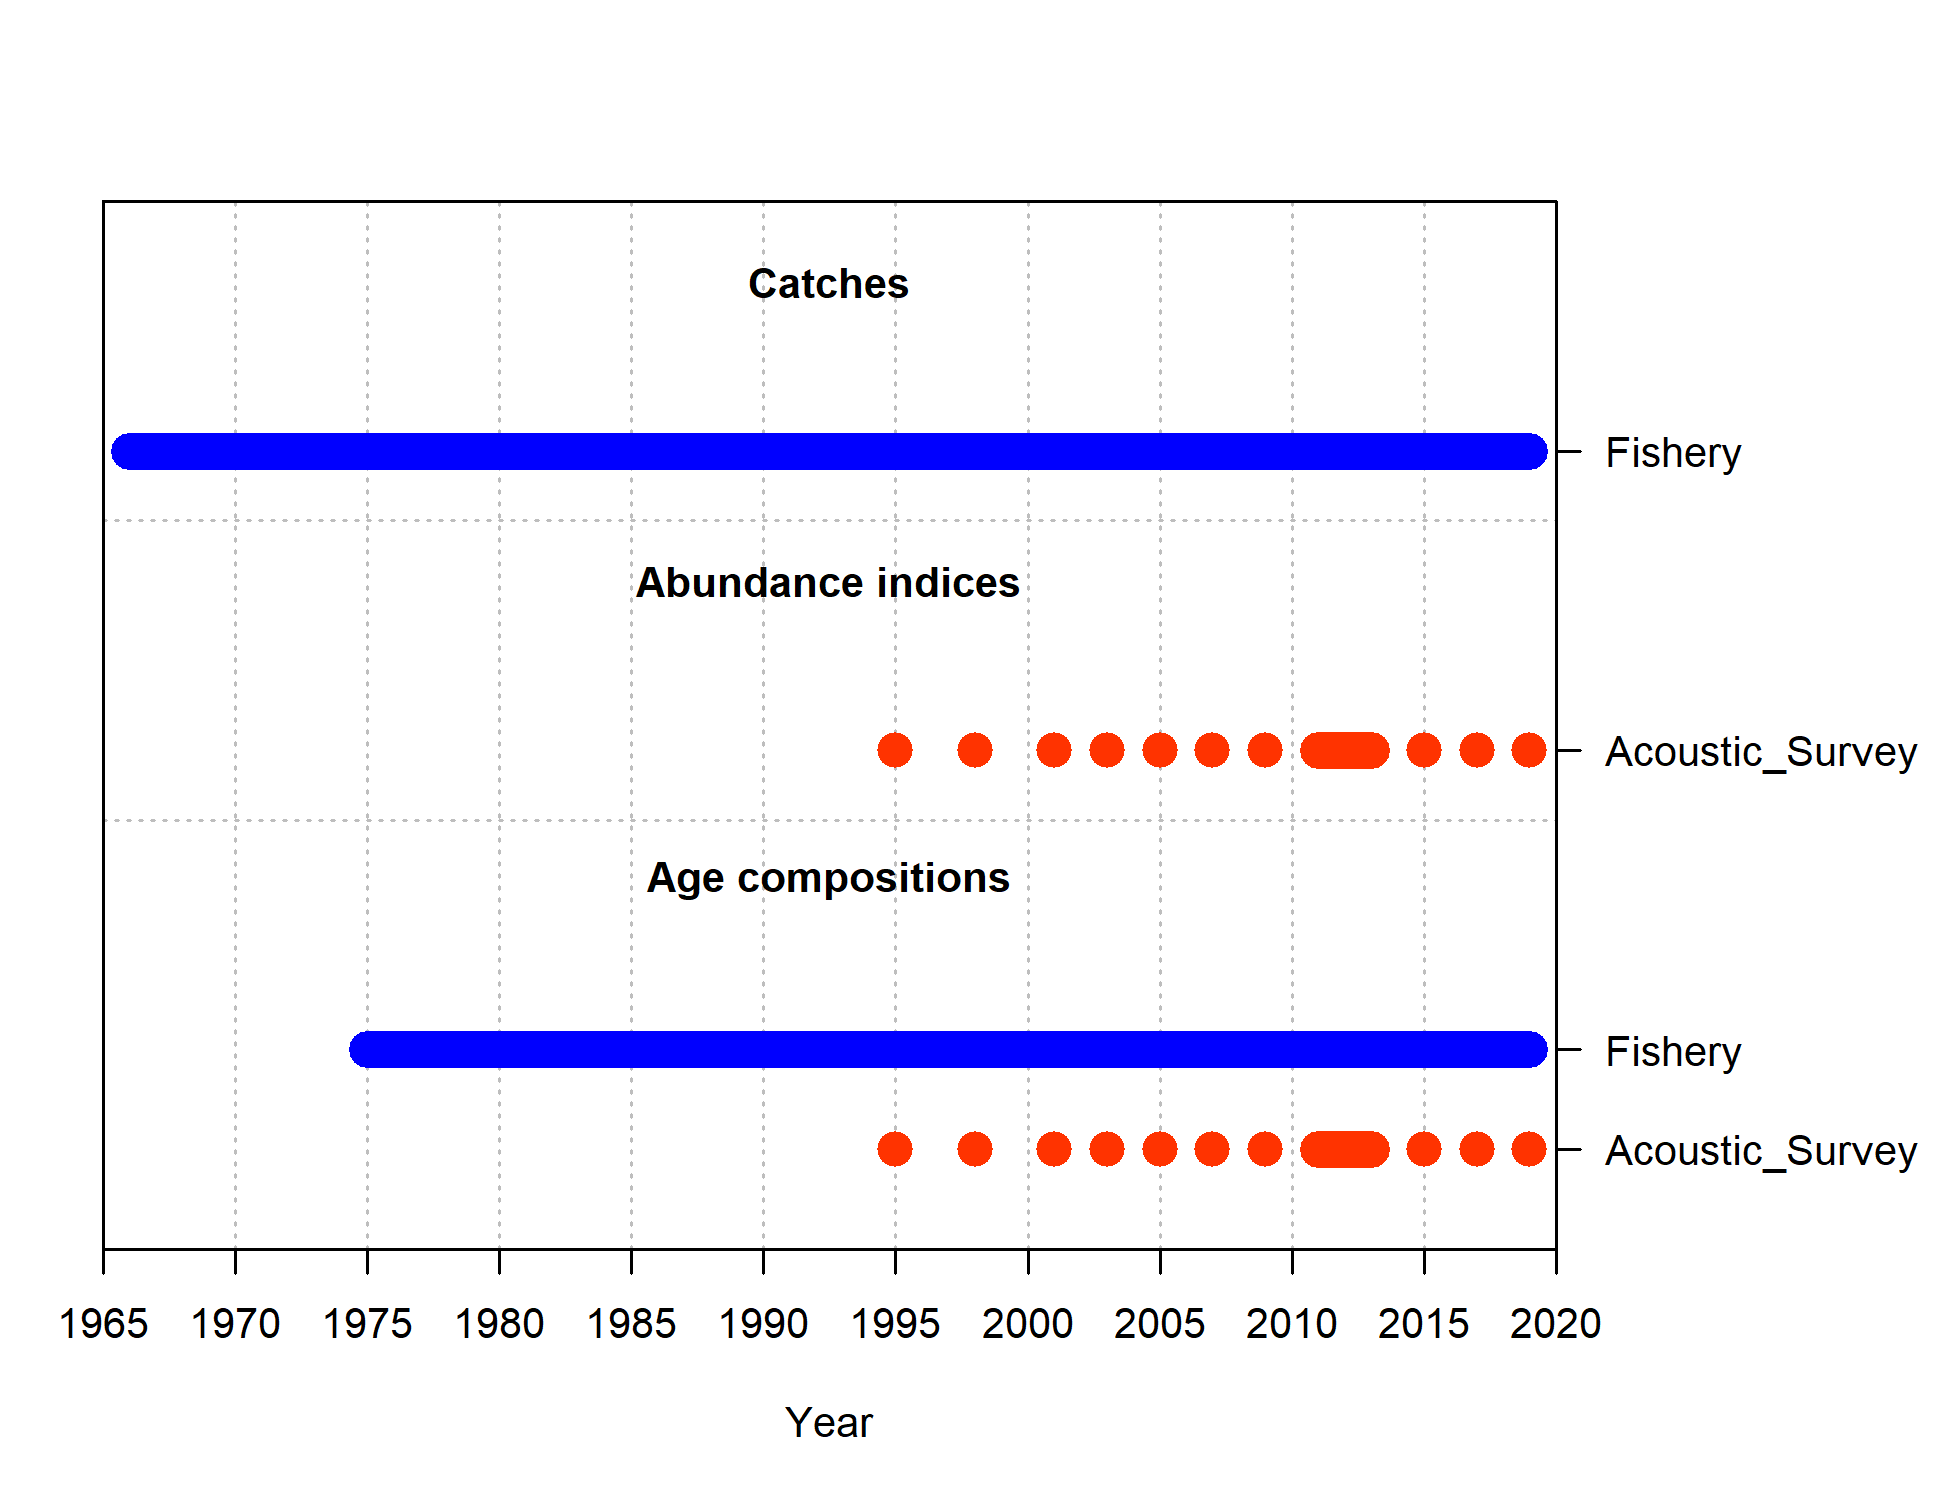
\includegraphics[width=1\textwidth,height=1\textheight]{data-plot.png}
\caption{Summary of data sources used in the base model.\label{fig:data-plot}}
\end{figure}
\end{document}
